% ============================================================
% CHAMPS -- Icing Framework
% ============================================================

\begin{frame}[c]{\small CHAMPS -- Icing Framework}
\scriptsize

\centering

% ------------------------------------------------------------
% Icing Framework
% ------------------------------------------------------------

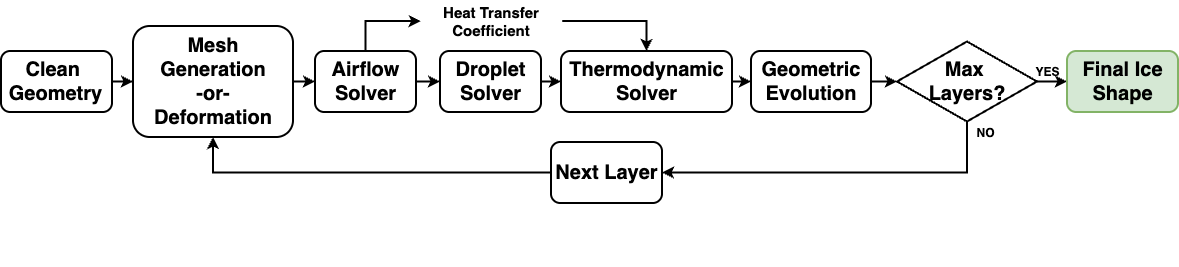
\includegraphics[
    width=0.88\textwidth,
    height=2.25cm,
    keepaspectratio
]{FIGURES/LS_FRAMEWORK/icingFramework.png}

\vspace{0.10cm}

% ------------------------------------------------------------
% Modeling Configuration
% ------------------------------------------------------------

\renewcommand{\arraystretch}{1.18}
\setlength{\tabcolsep}{5pt}

\begin{tabularx}{0.90\textwidth}{
    |>{\centering\arraybackslash}p{0.35\textwidth}
    |>{\centering\arraybackslash}X
    |>{\centering\arraybackslash}X|
}
\hline

\rowcolor{polymtlbluel}
\color{white}\textbf{Model / Method} &
\color{white}\textbf{NACA0012} &
\color{white}\textbf{ONERA M6} \\
\hline

Turbulence Model &
\multicolumn{2}{c|}{Spalart--Allmaras (SA)} \\
\hline

Heat-Transfer Method &
\multicolumn{2}{c|}{One Solution + $T_{\mathrm{rec}}$} \\
\hline

Droplet Model &
\multicolumn{2}{c|}{Eulerian / Lagrangian} \\
\hline

Droplet Drag Model &
\multicolumn{2}{c|}{Deformable Sphere} \\
\hline

SLD Corrections &
\multicolumn{2}{c|}{None} \\
\hline

Thermodynamic Model &
\multicolumn{2}{c|}{Messinger} \\
\hline

Ice Density &
$580~\mathrm{kg/m^3}$ &
$680~\mathrm{kg/m^3}$ \\
\hline

Surface Roughness &
$0.2667$ mm / $0.5334$ mm &
$1.0$ mm \\
\hline

Geometry Evolution &
\multicolumn{2}{c|}{Algebraic (Single-shot) / Level Set (Multilayer)} \\
\hline

Accretion Strategy &
\multicolumn{2}{c|}{Single-shot \& 5 Layers} \\
\hline

\end{tabularx}

\vspace{0.08cm}

% ------------------------------------------------------------
% Numerical Details
% ------------------------------------------------------------

\begin{flushleft}
\tiny
\textbf{*} Flow equations use Roe convective fluxes with the
Venkatakrishnan limiter; Eulerian droplet equations use an upwind
scheme with the Van Albada limiter. Lagrangian simulations were
performed to verify the Eulerian collection-efficiency predictions.
\end{flushleft}

\end{frame}

% ============================================================
% CHAMPS -- MULTILAYER ICE-ACCRETION APPROACH
% ============================================================

\begin{frame}[c]{\small CHAMPS -- Multilayer Ice-Accretion Approach}
\scriptsize

\vspace{-0.10cm}

\centering

% ============================================================
% LEFT -- LEVEL-SET FORMULATION
% ============================================================
\begin{minipage}[t]{0.40\textwidth}
\vspace{0pt}

\begin{block}{\scriptsize Level-Set Formulation}

The ice--air interface is implicitly represented by the
\textbf{zero level set} of a signed-distance function $\phi$
\cite{OSHER2004,FROLKOVIC2015214,lavoieLevelSet}:

\vspace{-0.10cm}

\[
\frac{\partial \phi}{\partial t}
+ \nabla \cdot (\phi \boldsymbol{V})
- \phi \nabla \cdot \boldsymbol{V}
= 0,
\qquad
\boldsymbol{V}
=
\frac{h_{\mathrm{ice}}}{\Delta t_{\mathrm{layer}}}
\,\boldsymbol{n}_{\phi_0}.
\]

\vspace{-0.10cm}

\begin{itemize}
    \setlength{\itemsep}{0.45cm}

    \item $\boldsymbol{n}_{\phi_0}$ denotes the local level-set normal
    computed from the initial wall-distance field $\phi_0$.

    \item The predicted ice thickness defines the interface advection velocity
    $\boldsymbol{V}$.

    \item The interface is advected through unsteady time stepping
    until either the prescribed icing time or the predicted ice volume is reached.

    \item The updated ice geometry is extracted from the
    $\boldsymbol{\phi=0}$ isosurface using the open-source
    Mmg library \cite{dapogny2014mmg}, and used for the next accretion layer.

\end{itemize}

\end{block}

\end{minipage}%
\hspace{0.03\textwidth}%
% ============================================================
% RIGHT -- ILLUSTRATIONS
% ============================================================
\begin{minipage}[t]{0.50\textwidth}
\vspace{0pt}
\centering

% ------------------------------------------------------------
% Level-set / interface illustration
% ------------------------------------------------------------
\textbf{\scriptsize Ice--Air Interface}

\vspace{0.03cm}

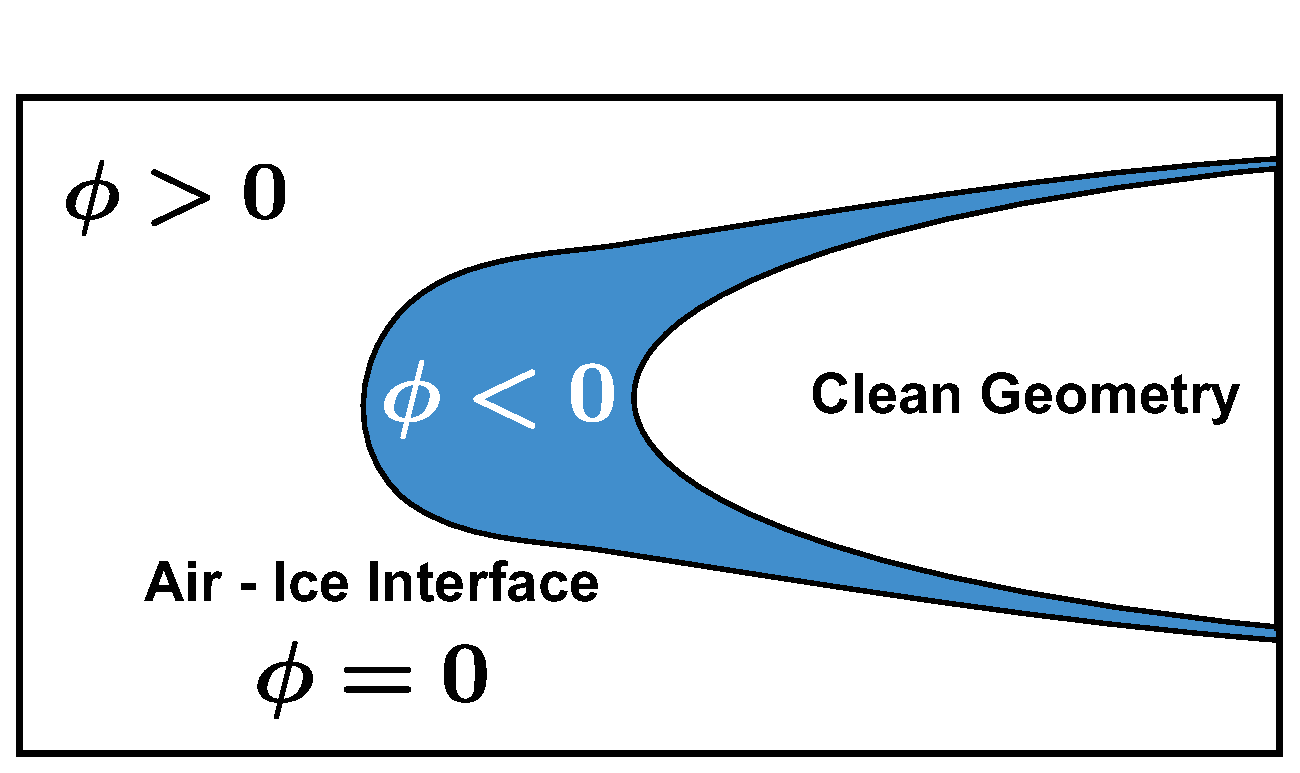
\includegraphics[
    width=\textwidth,
    height=2.65cm,
    keepaspectratio
]
{FIGURES/LS_FRAMEWORK/ICE_AIR_INTERFACE.eps}

\vspace{0.12cm}

% ------------------------------------------------------------
% Complex 3D ice geometry
% ------------------------------------------------------------
\textbf{\scriptsize Extracted 3D Ice Geometry}

\vspace{0.03cm}

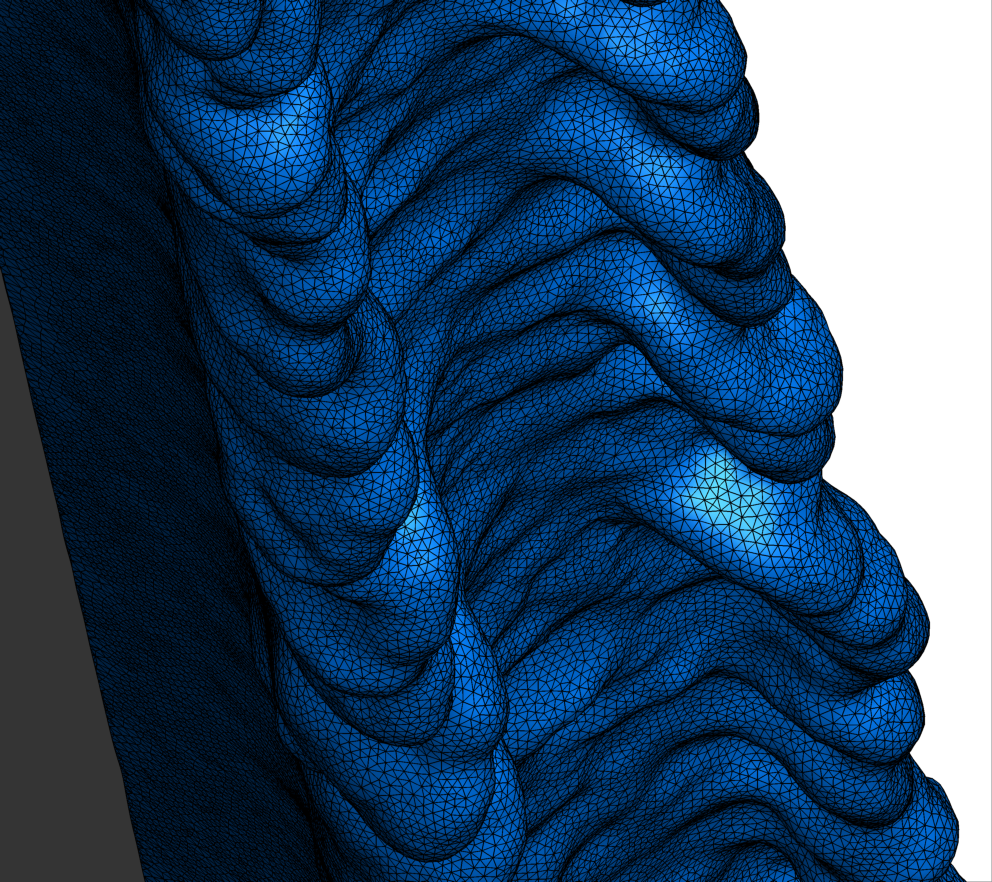
\includegraphics[
    width=\textwidth,
    height=4.05cm,
    keepaspectratio
]
{FIGURES/LS_FRAMEWORK/CLIPPED_ICE_SHAPE_CASE_362_3.png}

\end{minipage}

\end{frame}